\subsection{Learning-to-Search Summarizer}

\begin{frame}{Model Features}
  \begin{columns}
      \begin{column}{.5\textwidth}
      \begin{itemize}
        \item Surface Features
        \item Query Features
        \item Language Model Scores
        \item Single Document Summarization Rankings\\~\\ %(L2S)
        \item \only<1>{Nugget Probability} 
              \only<2->{\textbf{Nugget Probability}}
            \begin{itemize}
                \item<2->  N-gram classifier for 
                    predicting when a sentence contains a nugget.
            \end{itemize}
        %\item Geographic Relevance (SAP)
        %\item Temporal Relevance (SAP)
      \end{itemize}
    \end{column}
    \begin{column}{.5\textwidth}
      \begin{itemize}
          \item \only<1-2>{Document Frequency}
                \only<3->{\textbf{Document Frequency}}
            \begin{itemize} %(L2S)
                \item<3-> Hour-to-hour relative change in number of documents 
                    in the stream.
            \end{itemize}~\\~\\
        %\item Stream Language Model Scores %(L2S)
        \item \only<1-3>{ Update Similarity}
           \only<4->{\textbf{Update Similarity}} %(L2S)
             \begin{itemize}
                \item<4-> Similarity of candidate sentence extract to all 
                    previously extracted sentences.
             \end{itemize}
%        \item Nugget Probability %(L2S)
%        \item Single Document Summarization Rankings %(L2S)
      \end{itemize}
   \end{column}
  \end{columns}
\end{frame}




\begin{frame}{Learning-to-Search Summarization}

 \begin{itemize}
   \item Nugget Probability model learned ``offline.'' 
   \begin{itemize}
     \item I.e. doesn't take into account future extraction decisions, or 
           account for compounding error.
     \item It's difficult to take into account summary features.
   \end{itemize}
   \item<4-> Learning-to-search (Daum\'e, Langford, and Marcu (2009)), effectively an exploration/data sampling scheme
       can correct for this!
 \end{itemize}

    \begin{center}
    \only<1-2>{
        \uncover<2>{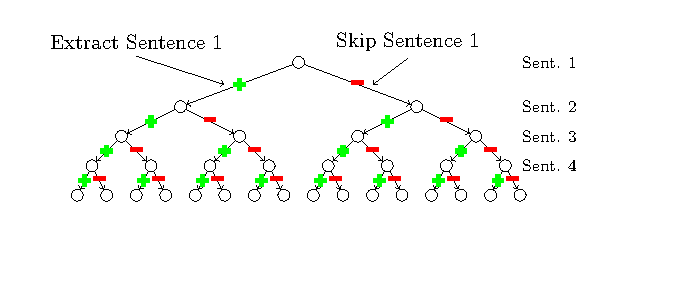
\includegraphics[scale=.7]{2_feature_based_models_of_salience/image_texs/l2s1/l2s1.pdf}}
    }
    \only<3>{
    
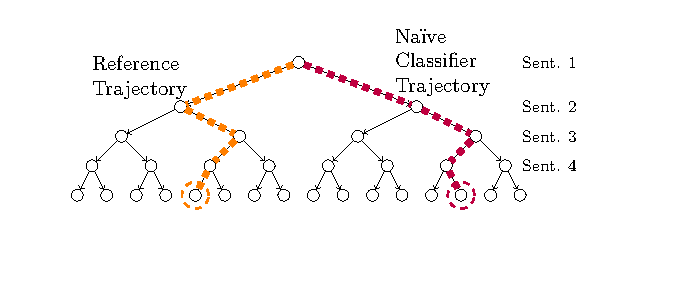
\includegraphics[scale=.7]{2_feature_based_models_of_salience/image_texs/l2s2/l2s2.pdf}}
    \only<4>{
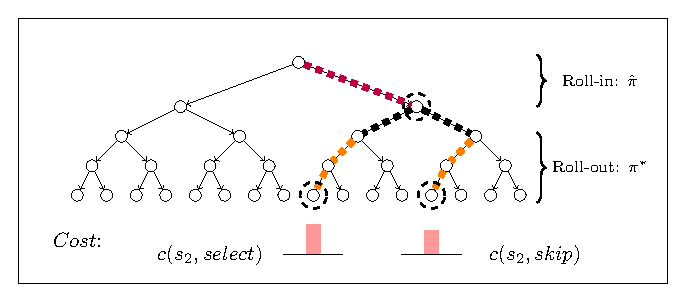
\includegraphics[scale=.7]{2_feature_based_models_of_salience/image_texs/l2s3/l2s3.pdf}}
\end{center}
\end{frame}



\begin{frame}{Experiments}

    \begin{itemize}
    \item Leave-One-Out evaluation
        \begin{itemize}
            \item 44 TREC 2015 Temporal Summarization events.\\~\\
            \item 5 queries randomly selected for development set.\\~\\
            \item Leave-One-Out Evaluation on remaining 39 events.\\~\\
        \end{itemize}
    \end{itemize}


\end{frame}
\begin{frame}
    \frametitle{Evaluation Metrics}
    \begin{itemize}
      %  \item \textsc{Rouge}
       % \begin{itemize}
       %     \item ``reference'' summary generated by concatenating event 
       %             nugget texts
       % \end{itemize}
%~\\
    \item TREC Temporal Summarization metrics~\\~\\
        \begin{itemize}
            \item  \textbf{Expected Gain} --- the average number of novel nuggets in 
                each extracted sentence; $\approx$ nugget precision. ~\\~\\
            \item \textbf{Comprehensiveness} --- nugget recall.
        \end{itemize}
%    \item Expected Gain and Comprehensiveness
%        $$\mathbb{E}[\mathrm{Gain}] = \frac{|S_n|}{|S|}\;\;\;\;\;\;\;\;\;
%            \textrm{Comprehensiveness} = \frac{|S_n|}{|N|}$$
%            where \begin{itemize}
%            \item[] $S$ is the set of system updates
%                \item[] $S_n$ is the set of nuggets mapped to updates in $S$
%                \item[] $N$ is the set of nuggets for the event
%            \end{itemize}
    \end{itemize}
\end{frame}


\begin{frame}{System Comparisons}

  \begin{itemize}
    \item \textbf{Baseline Models}

    \begin{itemize}
        \item \textbf{Cos} --- Cosine Similarity Threshold
        \begin{itemize}
            \item Selects sentence if it's max similarity to any previous 
                  update is below a threshold.
            \item Only examines first sentences of article. 
        \end{itemize}
      \item \textbf{AP} --- Affinity Propagation Clustering
    \end{itemize}~\\
    \item \textbf{Our Models}
    \begin{itemize}
      \item \textbf{SAP} ---  Salience-Biased Affinity Propagation Clustering 
      \item \textbf{L2S} --- Learning to Search 
      \item \textbf{L2SCos} --- Learning to Search with cosine similarity 
                                threshold
    \end{itemize}
  \end{itemize}

\end{frame}

\begin{frame}{Results}
\centering
%\only<1>{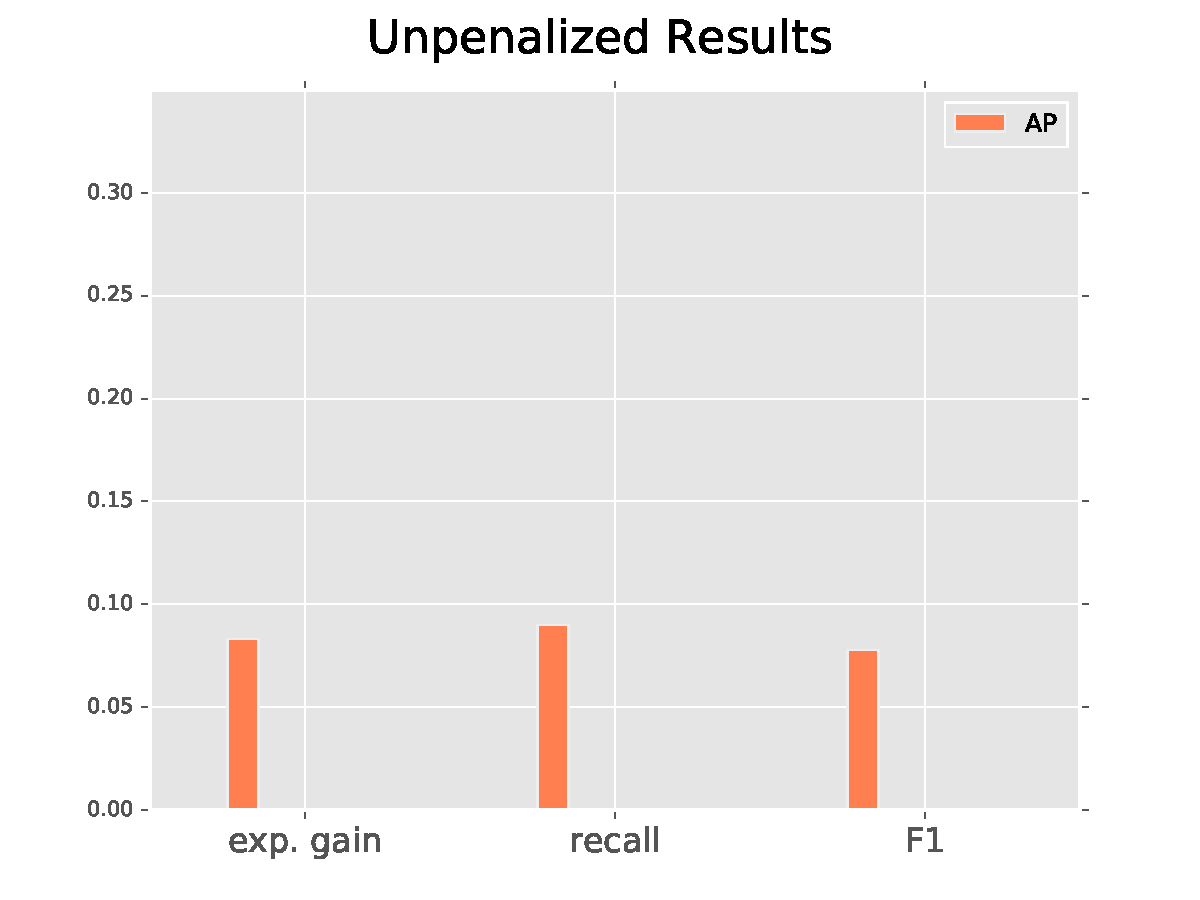
\includegraphics[scale=.45]{images/section2/uresults1.pdf}}
%\only<2>{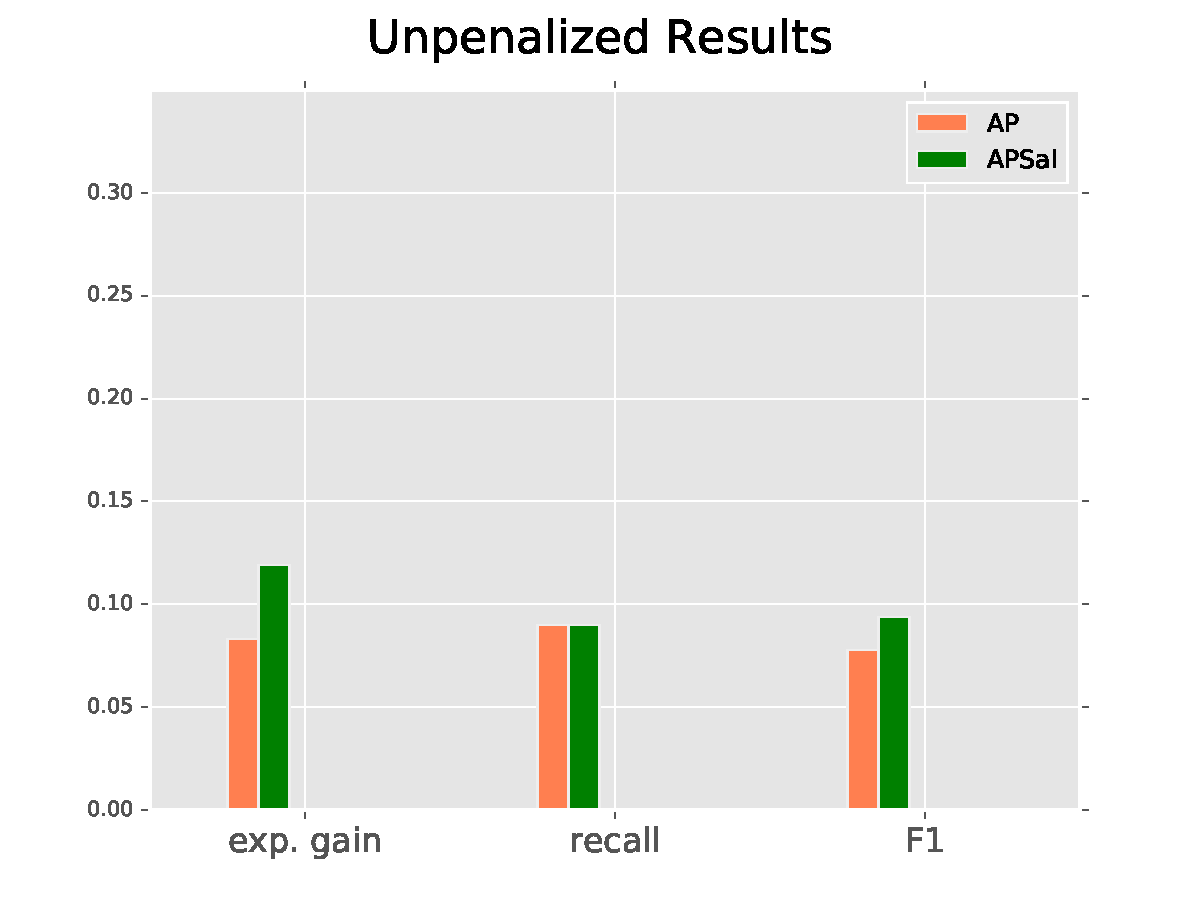
\includegraphics[scale=.45]{images/section2/uresults2.pdf}}
\only<1>{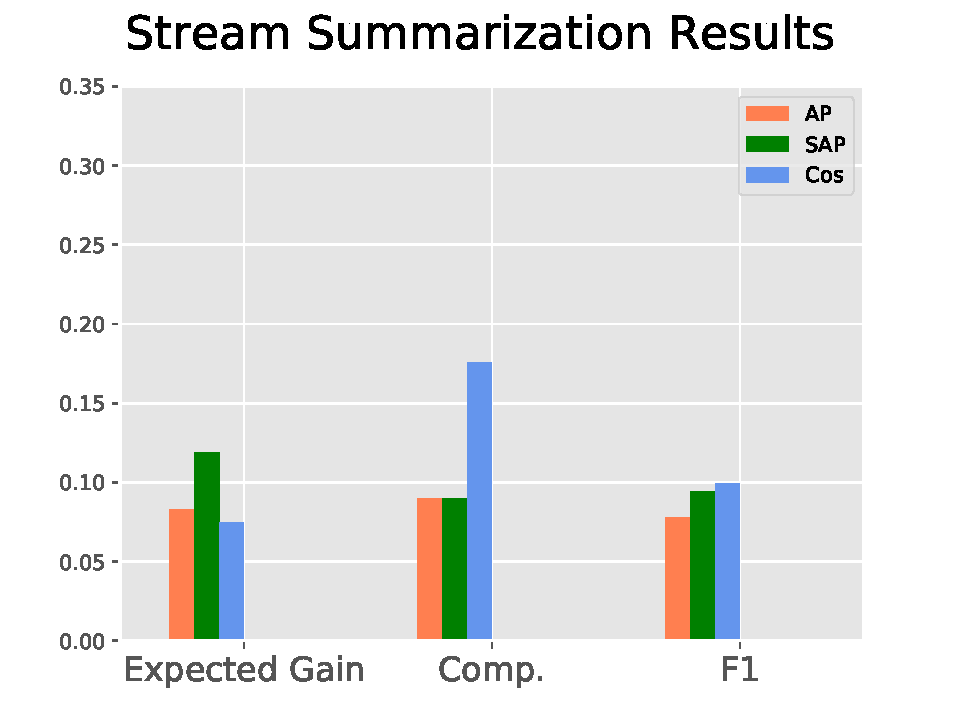
\includegraphics[scale=.45]{2_feature_based_models_of_salience/image_texs/results/uresults3.pdf}}
\only<2>{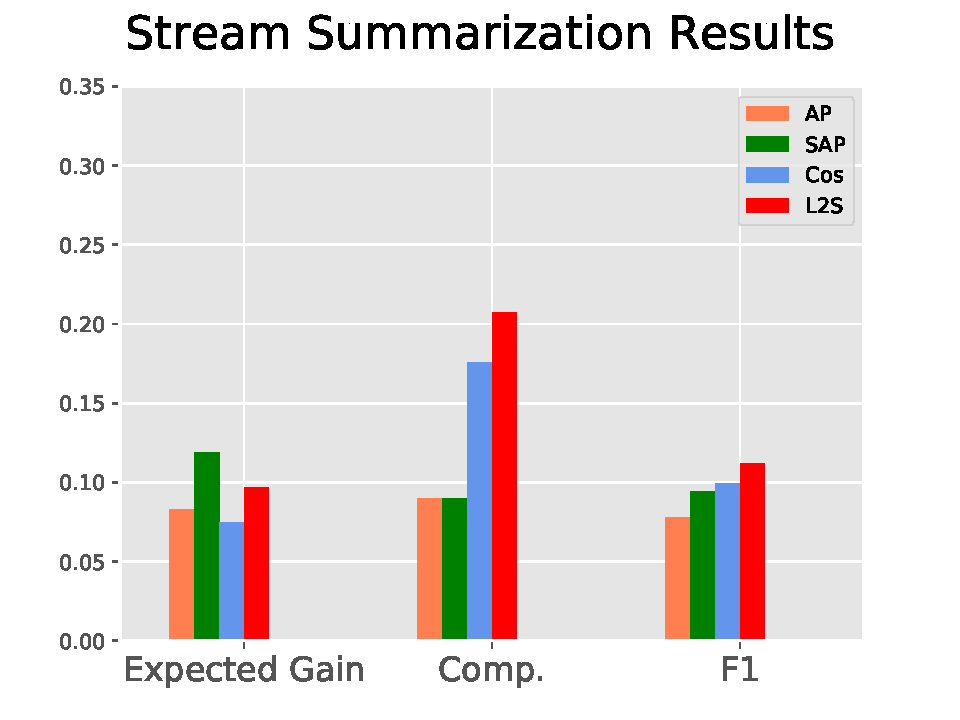
\includegraphics[scale=.45]{2_feature_based_models_of_salience/image_texs/results/uresults4.pdf}}
\only<3>{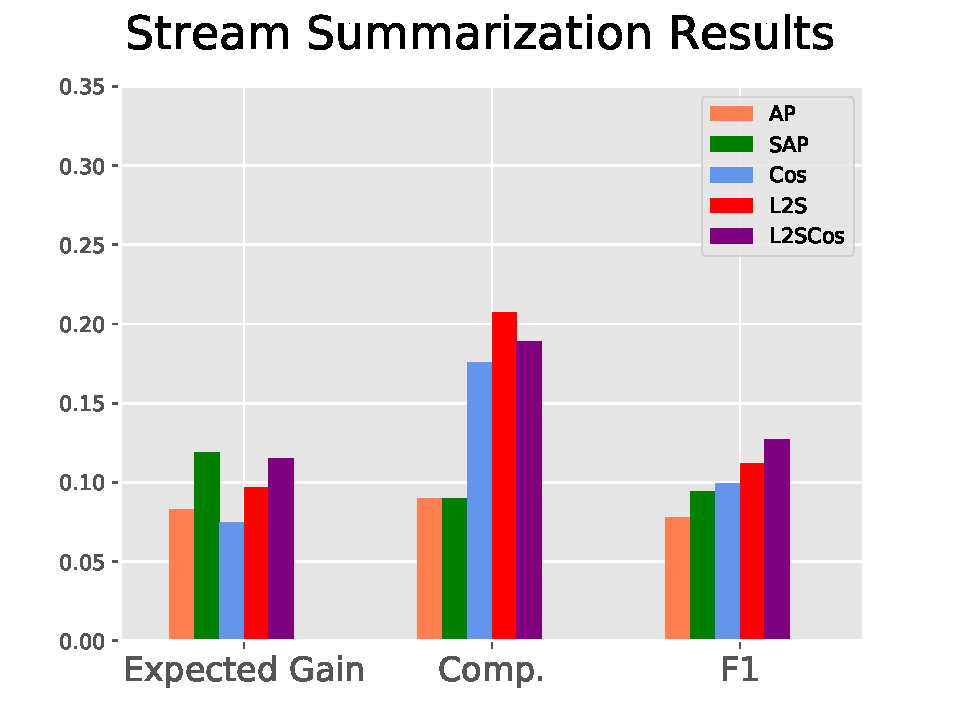
\includegraphics[scale=.45]{2_feature_based_models_of_salience/image_texs/results/uresults5.pdf}}

\end{frame}

\begin{frame}{Stream Summarization Takeaways}
    \begin{itemize}
        \item Learning-to-Search approach can beat tough lead-based baseline.~\\~\\

        \item Dynamic summary features important for achieving performance.
    \end{itemize}
\end{frame}
